% The bakery's feasible polygon and the simplex path (generated by figs_c2ch07.py).
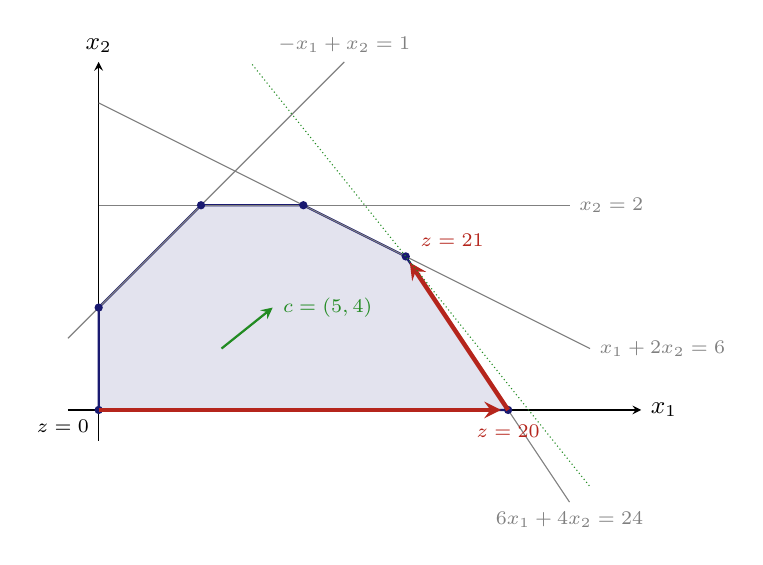
\begin{tikzpicture}[x=1.3cm,y=1.3cm,every node/.style={font=\small},>=stealth]
\draw[->] (-0.3,0) -- (5.3,0) node[right] {$x_1$};
\draw[->] (0,-0.3) -- (0,3.4) node[above] {$x_2$};
\fill[MidnightBlue!12] (0,0) -- (4,0) -- (3,1.5) -- (2,2) -- (1,2) -- (0,1) -- cycle;
\draw[MidnightBlue,thick] (0,0) -- (4,0) -- (3,1.5) -- (2,2) -- (1,2) -- (0,1) -- cycle;
\draw[black!50] (3.5,0.75) -- (4.6,-0.9) node[below,font=\scriptsize] {$6x_1+4x_2=24$};
\draw[black!50] (0,3) -- (4.8,0.6) node[right,font=\scriptsize] {$x_1+2x_2=6$};
\draw[black!50] (-0.3,0.7) -- (2.4,3.4) node[above,font=\scriptsize] {$-x_1+x_2=1$};
\draw[black!50] (0,2) -- (4.6,2) node[right,font=\scriptsize] {$x_2=2$};
\fill[MidnightBlue] (0,0) circle (1.5pt);
\fill[MidnightBlue] (4,0) circle (1.5pt);
\fill[MidnightBlue] (3,1.5) circle (1.5pt);
\fill[MidnightBlue] (2,2) circle (1.5pt);
\fill[MidnightBlue] (1,2) circle (1.5pt);
\fill[MidnightBlue] (0,1) circle (1.5pt);
\draw[->,line width=1.6pt,BrickRed] (0,0) -- (3.93,0);
\draw[->,line width=1.6pt,BrickRed] (4,0) -- (3.04,1.44);
\node[below left,font=\scriptsize] at (0,0) {$z=0$};
\node[below,font=\scriptsize,BrickRed] at (4,-0.05) {$z=20$};
\node[above right,font=\scriptsize,BrickRed] at (3.05,1.5) {$z=21$};
\draw[->,thick,ForestGreen] (1.2,0.6) -- (1.2+0.5*1.0,0.6+0.4*1.0) node[right,font=\scriptsize] {$c=(5,4)$};
\draw[ForestGreen,densely dotted] (1.5,3.375) -- (4.8,-0.75);
\end{tikzpicture}
